\documentclass[crop,border=2pt]{standalone}

\usepackage{mathtools}
\usepackage{tikz}
\usetikzlibrary{positioning,scopes,arrows,shapes,decorations.pathreplacing}

\begin{document}
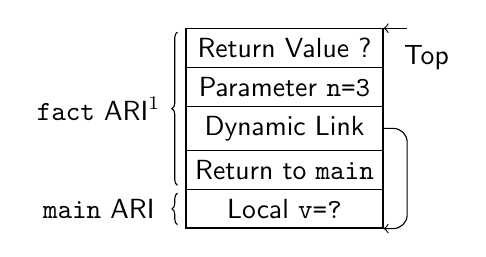
\begin{tikzpicture}[font=\sffamily,
  mystack/.style={rectangle split,rectangle split parts=#1,draw,anchor=center},
  myline/.style={->, rounded corners=5pt},
  mydec/.style={decorate,decoration={brace,amplitude=2pt}}]

  \node[mystack=5] (stk) {
    Return Value ?
    \nodepart{two} Parameter \texttt{n=3}
    \nodepart{three} Dynamic Link
    \nodepart{four} Return to \texttt{main}
    \nodepart{five} Local \texttt{v=?}
  };

  \draw[myline] (stk.three east) -- ([xshift=.3cm]stk.three east) -- ([xshift=.3cm]stk.south east) -- (stk.south east);

  \node [right=2.5cm of stk.text] (top) {Top};
  \draw[myline] ([xshift=.3cm]stk.north east) -- (stk.north east);

  \draw[mydec] ([xshift=-.1cm,yshift=.5mm]stk.four split west) --
               ([xshift=-.1cm,yshift=-.5mm]stk.north west) node [black,midway,xshift=-1cm] {\texttt{fact} ARI\(^{1}\)};
  \draw[mydec] ([xshift=-.1cm,yshift=.5mm]stk.south west) --
               ([xshift=-.1cm,yshift=-.5mm]stk.four split west) node [black,midway,xshift=-1cm] {\texttt{main} ARI};

\end{tikzpicture}
\end{document}
